
\subsection{Application on AIG Datas}
\label{sec:appl-aig-datas}
\paragraph{}
In this section we will apply the previous results on quoted spreads data of the
company  AIG. The  data provided  is  a series  of  CDS quoted  spreads for  the
maturities $1,\dots,10$ between 16/08/2005 and 30/09/2010.

\subparagraph{}
The first  idea consist on studying  statistically the behavior of  spreads over
2005 - 2010. 

\begin{figure}[H]
  \centering 
  \includegraphics[width=0.8\textwidth]{dynamic_spreads}
  \caption{\it Evolution of spreads of the company AIG }
  \label{fig:5}
\end{figure}
\paragraph{}
We  can naturally  remark two  phases in  the spreads  evolution: the  first one
corresponds  to a  stagnation of  CDS  market from  0 to  600 corresponding  to
16/08/2005-03/12/2007 .  The second one remains from the surrounding of 600 to
the end  of the period  30/09/2010. This period  is exactly superimposed  to the
subprime crisis. We  can remark that the  company have reached a  hight level of
spreads. This policy  is quite  natural in  a period of  crisis, the  company had  had to
increase her spreads in presence of a hight risk of bankruptcy. \\

\paragraph{}
In almost all  quotations, spread is an increasing function  of time. Obviously,
the more  years protection recover, higher  is the risk that  the protecter most
care. But how much  would the company be vulnerable to  maturity ? The following
graphic shows the spreads volatility over the available maturities :

\begin{figure}[H]
  \centering
\label{fig:6}
  \includegraphics[width=0.8\textwidth]{spreads_volatility}
  \caption{Quoted spreads volatility }
\end{figure}

The company in fact, in a crisis period, is too vulnerable to the maturity. 

\subsection{Dynamic of bounds }
\label{sec:dynamic-bounds-}

\paragraph{}
Under  \textit{arbitrage-free}  conditions, proposition  (\ref{prop:3.2})  gives
bounds for credit curves at each quotation :
\begin{figure}[H]

  \centering
  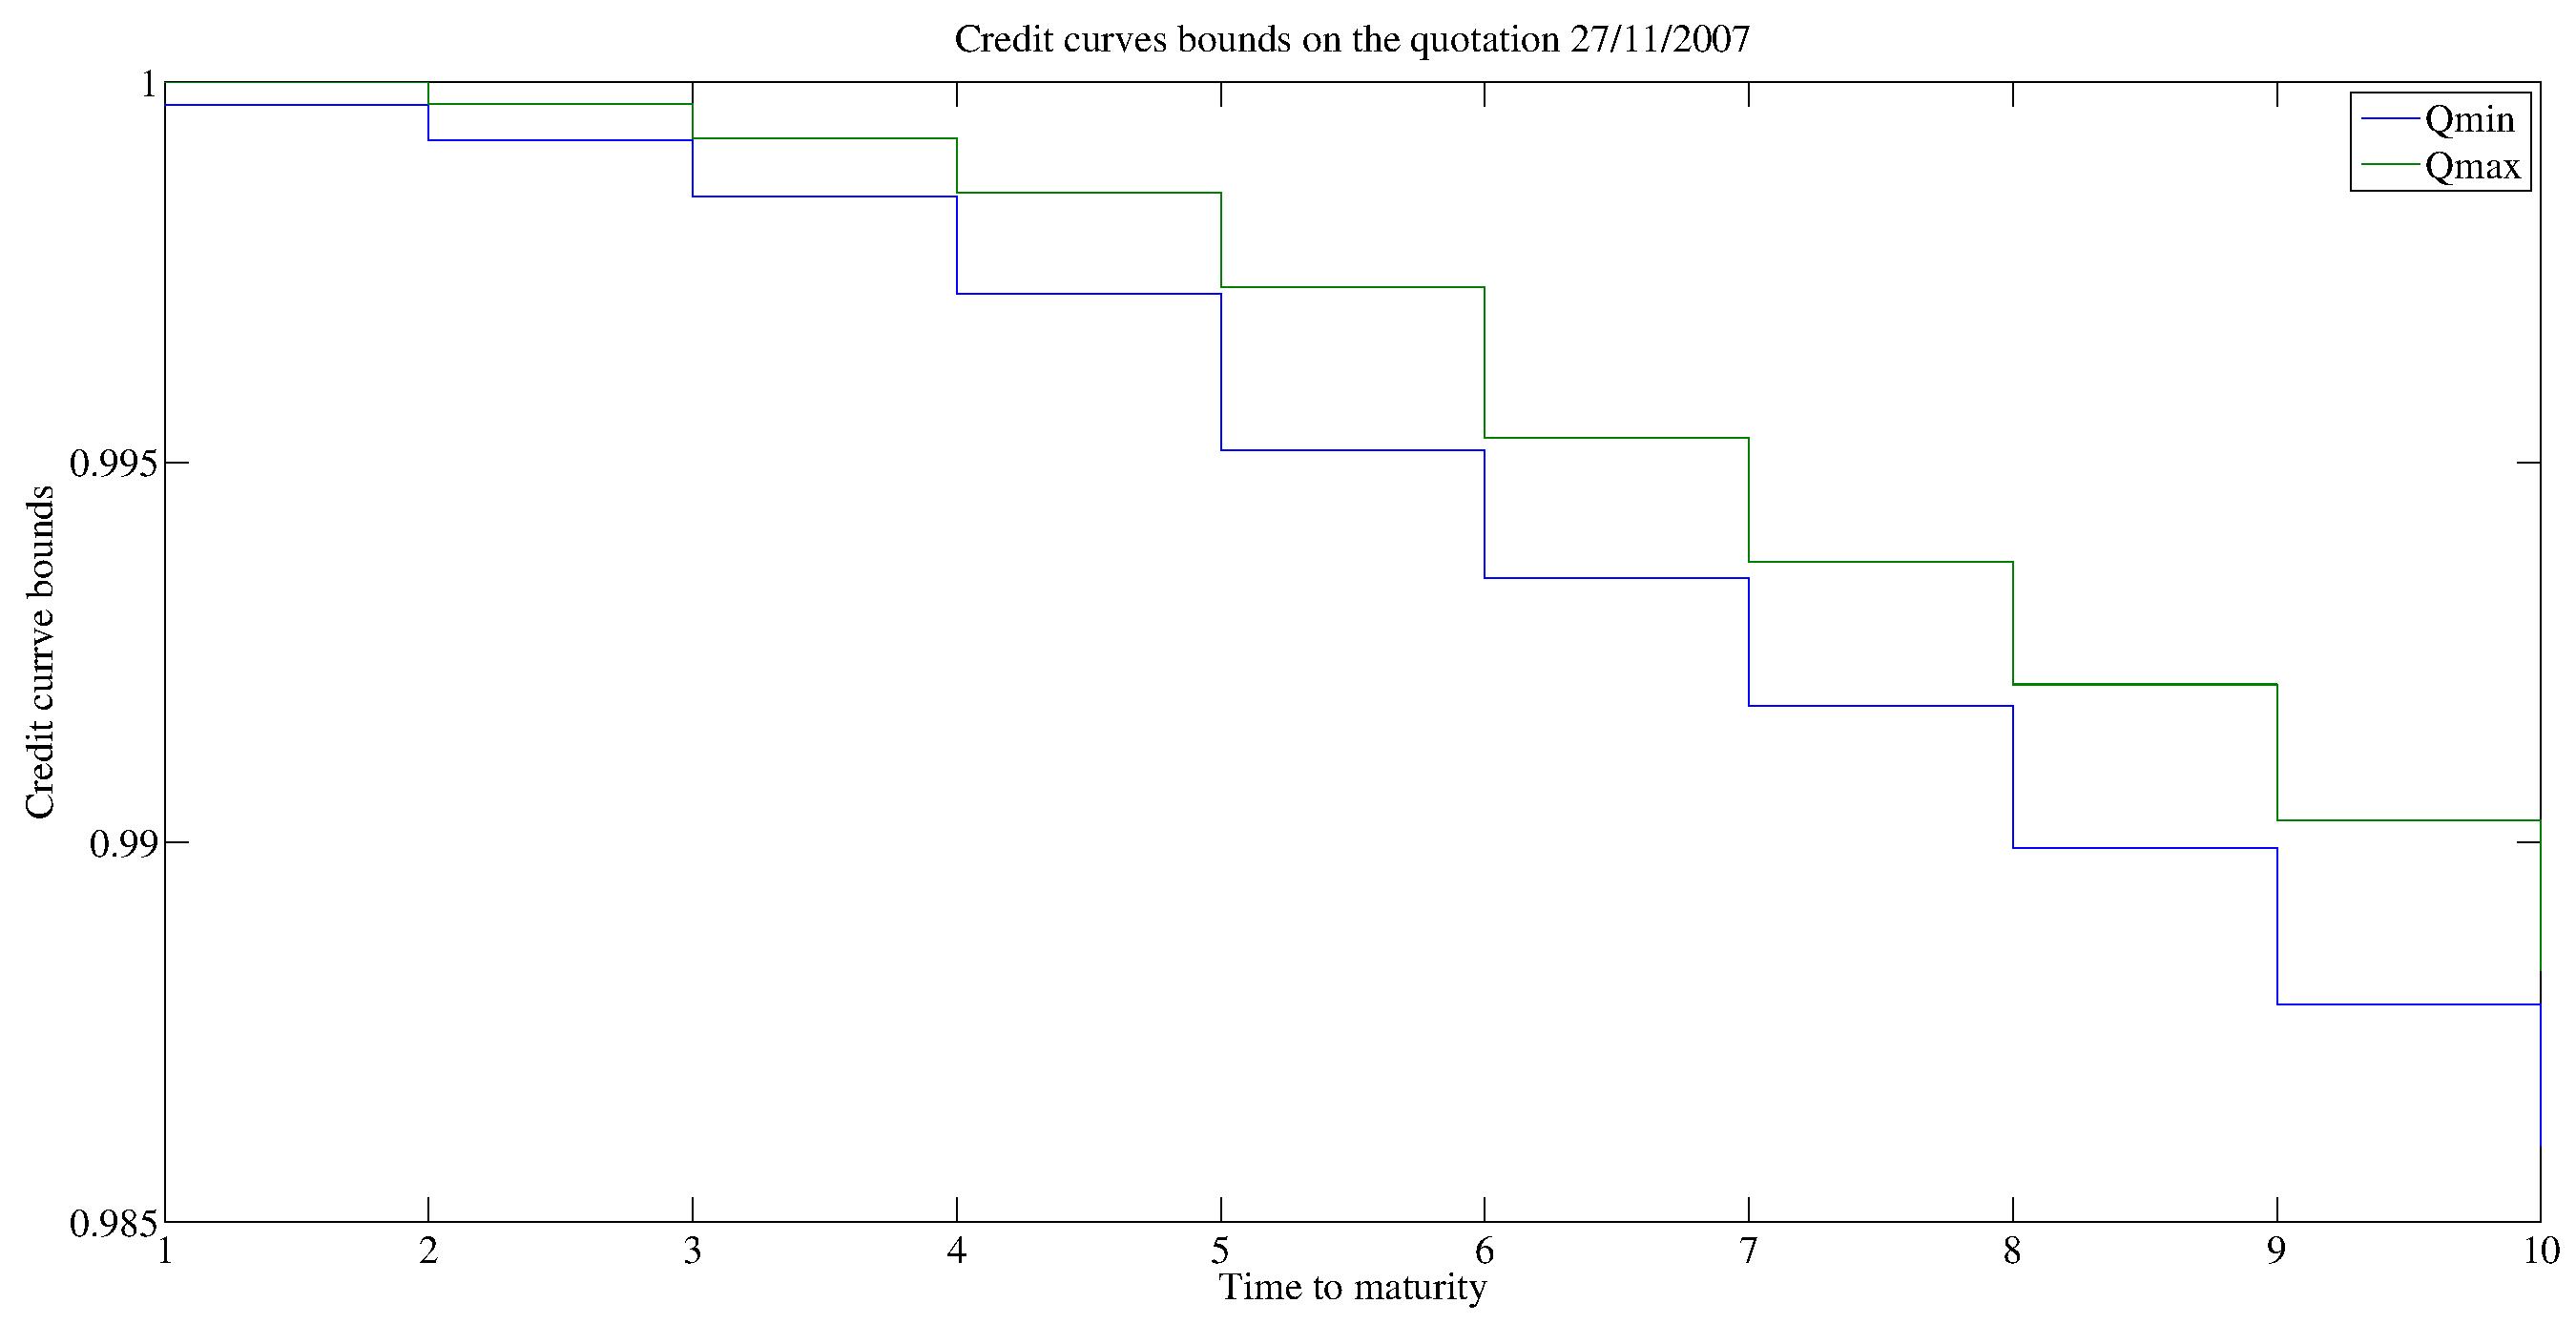
\includegraphics[width=0.8\textwidth]{cotation_27_11_2007}
  \caption{\it Credit curve among 18/08/2005 - 28/09/2007}
\label{fig7}
\end{figure}

We can  use this  proposition to
identify   either  arbitrage   free  opportunities   :  if   the  arbitrage-free
inequalities  are not  violated  that  means that  there  are  arbitrage at  the
specified quotation.  Indeed figure (\ref{fig:8}) shows an example of a quotation that
present an arbitrage opportunity :

\begin{figure}[H]
  \centering
  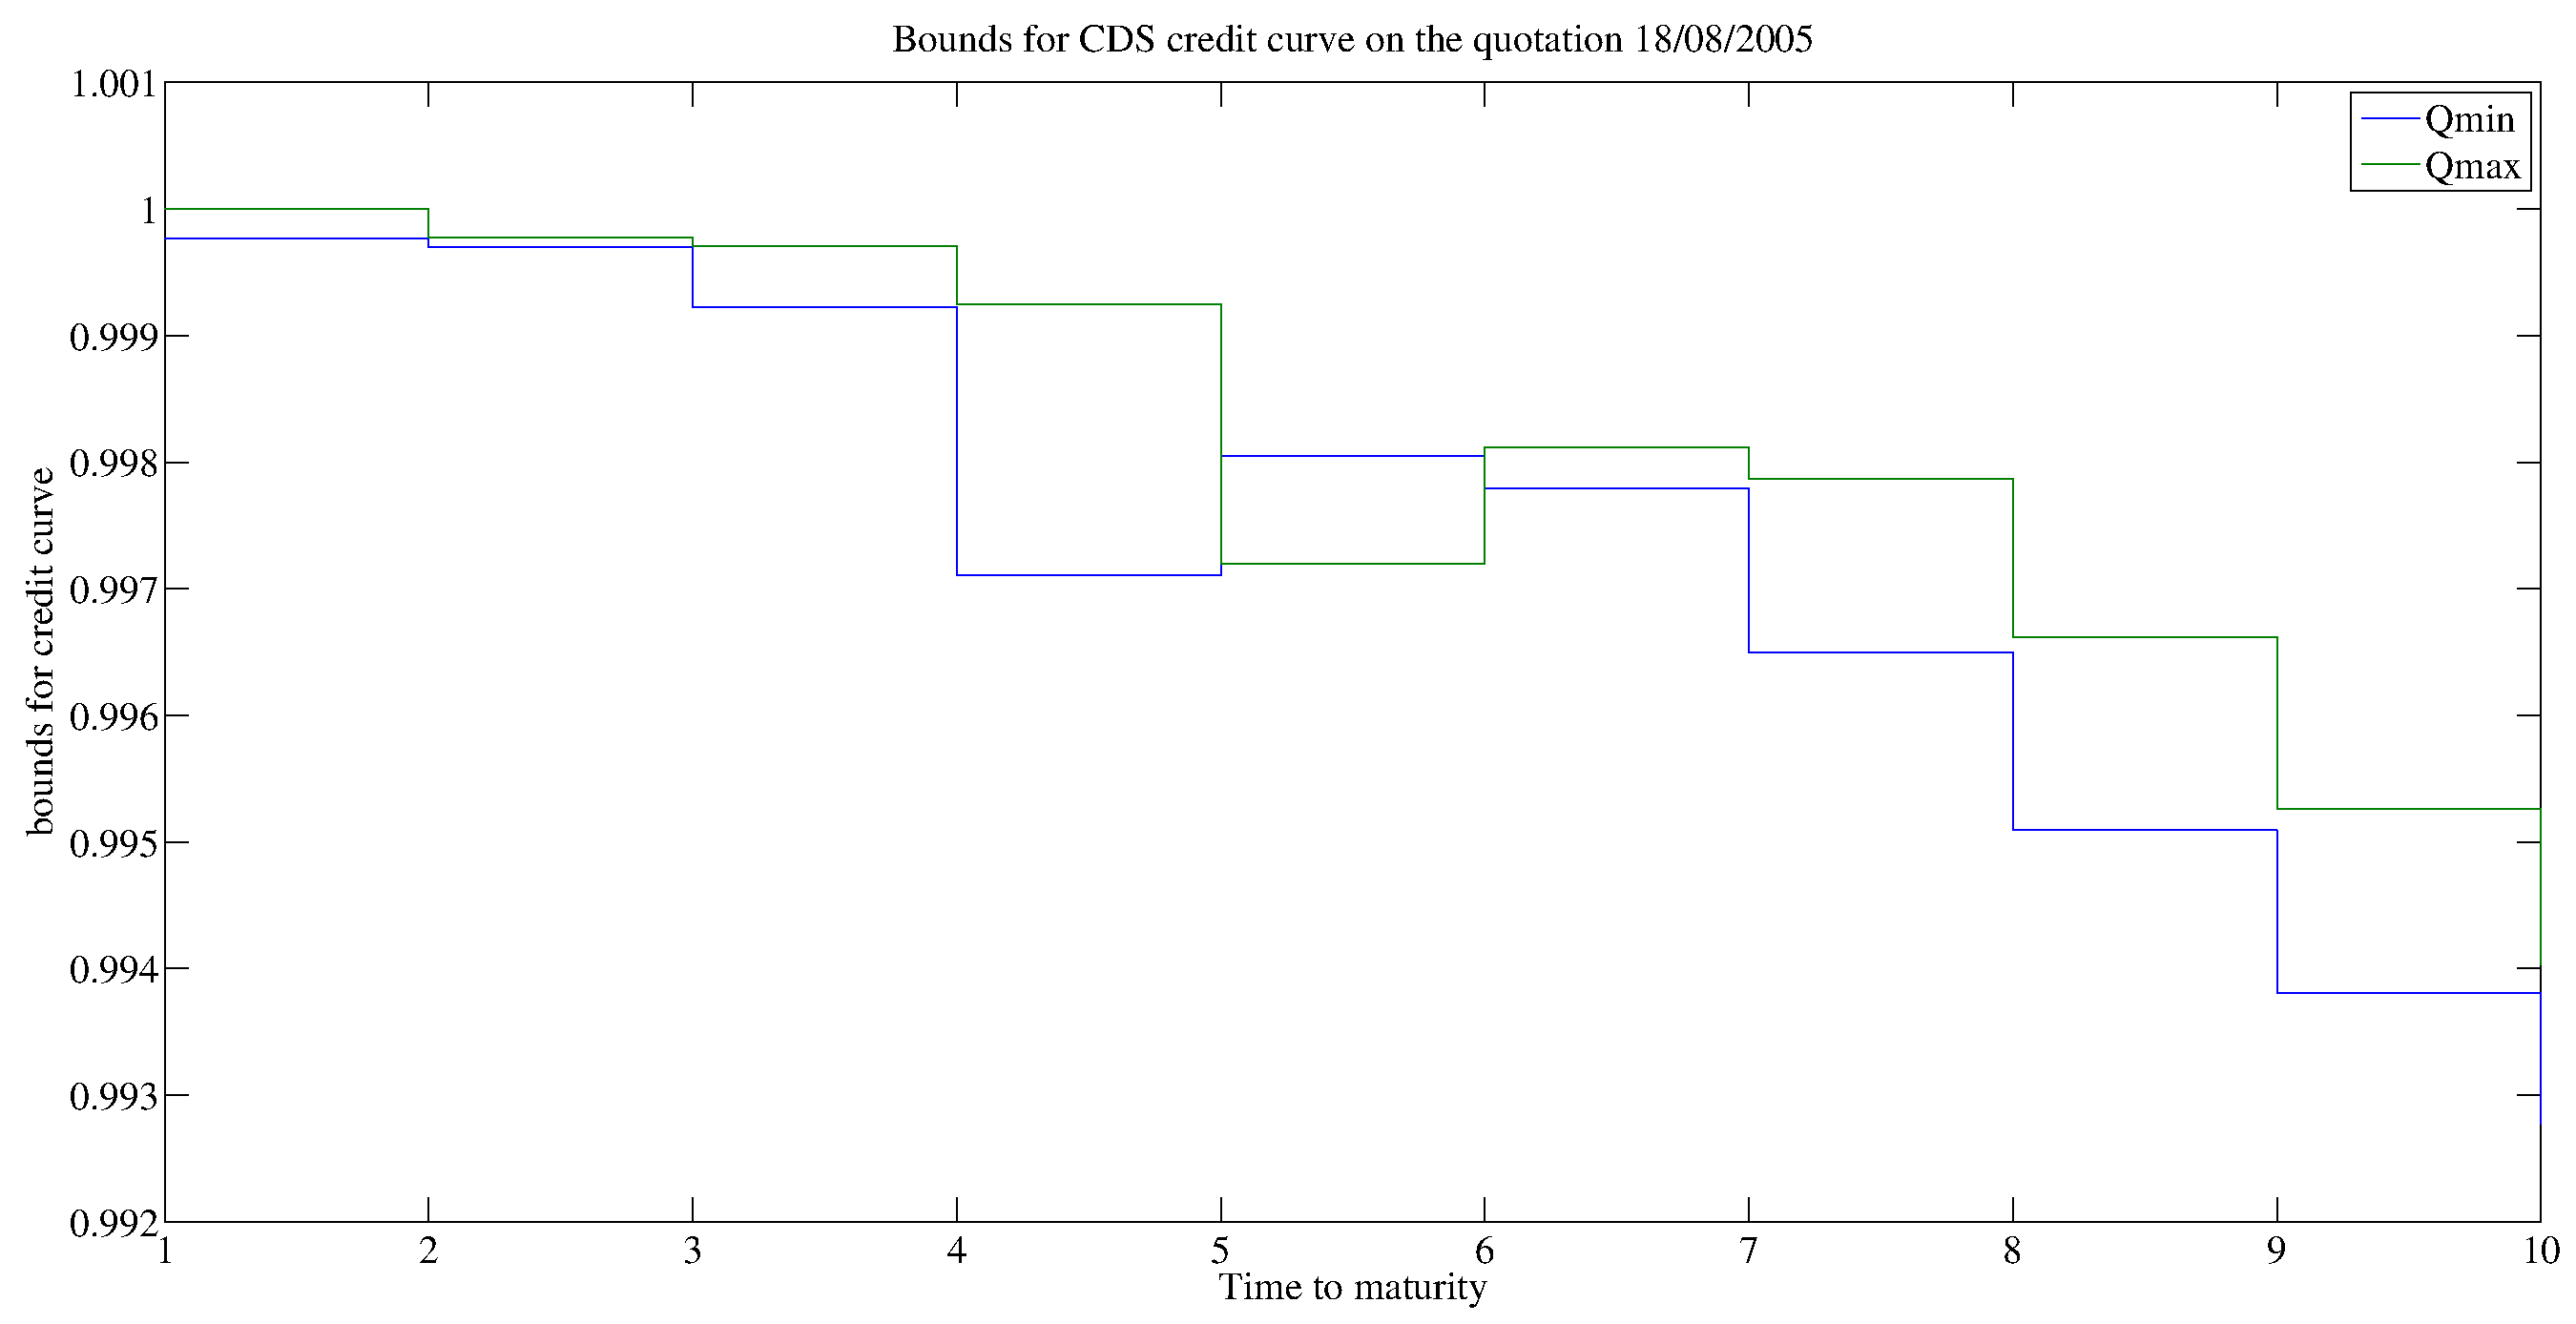
\includegraphics[width=0.8\textwidth]{cotation-18-08-2005}
  \caption{\it Market fit condition non verified}
  \label{fig:8}
\end{figure}


